\documentclass[]{report}
\usepackage{graphicx}
\usepackage{apacite}
\usepackage{times}
\usepackage{amssymb}
\usepackage{amsmath}
\usepackage{amsthm}
\usepackage{wrapfig}

%% Margin control
\textwidth 7.0in
\oddsidemargin -0.25in
\textheight 9.5in
\topmargin -0.75in

\begin{document}
\section*{Genthor}
\subsection*{Goal}
\setlength{\intextsep}{-40pt}
\begin{wrapfigure}[10]{r}{0.3\textwidth}
\vspace{-70pt}
%\begin{figure}[ht]
\centering
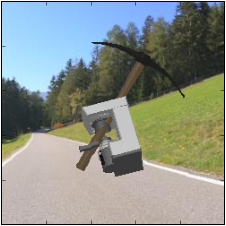
\includegraphics[width=0.3\textwidth]{example.png}
\caption{Example image}
%\label{fig:gen-model}
\end{wrapfigure}
%\end{figure}
\setlength{\intextsep}{40pt}

Developing a system for visual inference about naturalistic scenes
with multiple objects arranged in depth.

\subsection*{Definitions}
We focus on simple 3D scenes, $s \in \mathcal{S}$, that consist of a
background ($o_0$) that has a unique ID, $b$, and two spherical
rotation coordinates, $(r_{x,0}, r_{y,0})$, plus a set of foreground
objects ($n < 6$, for now) $(o_1,\dots,o_n)$. Each $o_i$ belongs to
one category, $c_i$, has 3 position coordinates,
$(p_{x,i},p_{y,i},p_{z,i})$, 3 scale coordinates,
$(w_{x,i},w_{y,i},w_{z,i})$, and 3 rotation coordinates,
$(r_{x,i},r_{y,i},r_{z,i})$.  The scene is unobserved, but it
generates images, $d \in \mathcal{D}$, through a rendering function,
$\mathrm{R}(\cdot)$, plus some noise, $\omega$.
\begin{align*}
  s &= (n,o_0,o_1,\dots,o_n)\\
  o_0 &= (b, r_{x,0}, r_{y,0})\\
  o_i &= (c_i, x_i,y_i,z_i, w_{x,i},w_{y,i},w_{z,i}, r_{x,i},r_{y,i},r_{z,i});\ i > 0\\
  d &= \mathrm{R}(s) + \omega
\end{align*}
We assume all values are discrete (for now).

\subsection*{Generative model}
Our assumed generative model specifies how scenes generate images
using prior and conditional probability distributions, $\Pr(S=s)$ and
$\Pr(D=d | S=s)$, to form a joint probability distribution that lets
us draw $(S,D)$ samples and evaluate their probabilities,
\[
\Pr(D=d,S=s) = \Pr(D=d | S=s)\Pr(S=s)
\]
We abbreviate $\Pr(X=x)$ as $\Pr(X)$.  Simple distribution assumptions
are:
\begin{align*}
  \Pr(S) &= \mathrm{Unif}(S)\\
  \Pr(D | S) &= \mathrm{Normal}(D; \mathrm{R}(S), \sigma_d)
\end{align*}

\subsection*{Inference}
Visual scene inference is defined as computing the Bayesian posterior
distribution,
\[
\Pr(S | D) = \frac{\Pr(D | S)\Pr(S)}{\sum_S \Pr(D | S)\Pr(S)}
\]
Since $\mathrm{R}^{-1}(D)$ is one-to-many and undefined, analytical
methods are hard to develop.  Monte Carlo sampling can be used to draw
posterior scene samples, $\{\tilde{S}_0,\dots,\tilde{S}_N\}$, which
support expectations, modes, density estimates, etc. Rejection or
importance sampling using proposals from the prior is inefficient
because the latent space is large. Instead, we use proposals drawn
from a feedforward discriminative model (Thor) to target high
probability of the latent space.

\subsubsection*{Thor (Dan -- fill in / correct)}
Thor is a system for feedforward visual recognition, based on
convolutional neural networks, that uses a sequences of nonlinear
filtering operations to compute a feature vector that supports linear
classification of objects. The input is a multichannel 2D image. Each
filtering step is composed of 5 sub-steps: 1. Linear filtering through
random projections, 2. Activation nonlinearity (sigmoid), 3. Pooling,
4. Normalization (optional), 5. Rescaling (subsampling). The output is
a feature vector(/tensor?), $F \in \mathcal{F}$, that is input to a
linear SVM. The training uses a sort of backpropagation (Is this
true?? how does it learn?).

Abstractly, Thor defines a map, $\mathrm{T}$, from images,
$\mathcal{D}$ to a set of feature vectors, $\mathcal{F}$, and a map,
$\tau_{\mathcal{P}}$, from $\mathcal{F}$ to the power set of $\mathcal{S}$,
$\mathcal{P}(\mathcal{S})$:
\begin{align*}
  \mathrm{T}(\cdot, \theta) &: \mathcal{D} \rightarrow \mathcal{F}\\
  \tau_{\mathcal{P}}(\cdot, \lambda) &: \mathcal{F} \rightarrow \mathcal{P}(\mathcal{S})
\end{align*}
where $\theta$ and $\lambda$ are parameters.

The parameters, $\theta$ and $\lambda$, are learned through training
on a set of virtual examples, $\{(D^{(k)}, S^{(k)});\ k=1, \dots,
K\}$, by minimizing the distances, $f(\cdot,\cdot)$, between scene
labels and predictions:
\begin{align*}
  \underset{\theta, \lambda}{\operatorname{argmin}} \sum_{k=1, \dots, K}
  f(S^{(k)}, \tau(\mathrm{T}(D^{(k)}, \theta), \lambda)
\end{align*}

Alternatively, Thor's $\tau$ can instead map to a measure, $e \in
\mathcal{E}$, of the strength of evidence for elements of $\mathcal{S}$, 
\begin{align*}
  \tau_{\mathcal{E}}(\cdot, \lambda) &: \mathcal{F} \rightarrow \mathcal{E}\\
  e &: \mathcal{S} \rightarrow \mathbb{R}^+
\end{align*}
which can then be transformed into an approximation of the posterior
over $S$:
\begin{align*}
  \Pr(S|D) \approx \frac{e(S)}{\sum_S e(S)}
\end{align*}

\subsubsection*{Rejection/importance sampling}
Thor's predicted approximate posterior can be used as a proposal
distribution for a rejection or importance sampling
algorithm. Specifically, the sampler's proposal distribution is,
\begin{align*}
  \mathrm{Q}(S) =
  \mathrm{Multinomial}\left(\frac{e(S)}{\sum_S e(S)} , n
  \right)
\end{align*}
where $n$ is the number of objects (which could also be predicted by
Thor).

For rejection sampling, the samples' acceptance probability is,
\begin{align*}
  a_j = \frac{\Pr(S_j | D)}{C \cdot \mathrm{Q}(S_j)}
\end{align*}
where $C$ is the rejection factor.

For importance sampling, the samples' (unnormalized) importances
weights are,
\[
w_j = \frac{\Pr(S_j | D)}{\mathrm{Q}(S_j)}
\]

\subsubsection*{Likelihood based on features}
In reality, 
\[
\Pr(D | S) \approx 
\begin{cases}
  1 , & \text{if } D = \mathrm{R}(S) \\
  0 , & \text{otherwise}
\end{cases}
\]
But generally, given $d$, $| \{s;\ d = \mathrm{R}(s), s \in
\mathcal{S} \} |$ is exponentially small in $|\mathcal{S}|$, so $\Pr(D
| S)$ does not support efficient Monte Carlo sampling.

We seek an approximation to $\Pr(D|S)$ that will make inference
easier.  Ideally, we'd find two distance measures,
\begin{align*}
  \rho & : \mathcal{D} \times \mathcal{D} \rightarrow \mathbb{R}^+ \\
  \rho' & : \mathcal{S} \times \mathcal{S} \rightarrow \mathbb{R}^+ 
\end{align*}
such that,
\begin{align*}
  \mathrm{abs} \left( \rho(\mathrm{R}(S_i), \mathrm{R}(S_j)) -
    \rho'(S_i, S_j) \right) < \epsilon \text{ ,}
\end{align*}
for small $\epsilon$.  Spearman rank correlation might be good.

An approximation that adds noise to the pixels might help soften the
posterior, but it does not necessarily fulfill the qualitative
isomorphism we need.

Our solution is to compose the Thor transform with the rendering
function and then assume (Gaussian) noise on the output features,
\begin{align*}
  \mathrm{R}^* = \mathrm{R} \circ \mathrm{T} : \mathcal{S} \rightarrow \mathcal{F}\\
  \Pr(F | S) = \mathcal{N}(F;S, \sigma_F)
\end{align*}

\end{document}